\titlespacing*{\section}
{0pt}{1ex plus 1ex minus .2ex}{-2.3ex plus .2ex}
\newcommand{\skipper}{\medskip\hrulefill\section{}}

\def \n {5} \def \radius {0.3\textwidth} \def \raz {1.4cm}    \def \radiusz {6.5cm}

\usetikzlibrary{shapes}

\tikzset{state/.style={circle, draw, inner sep=0.25cm, opacity=1, fill=black, minimum size=0.2pt}}

\tikzset{statez/.style={diamond,draw, thick, inner sep=0.1cm, opacity=1, fill=black, minimum size=0.2pt}}

\tikzset{statezz/.style={regular polygon,regular polygon sides=3,draw, thick, inner sep=0.08cm, opacity=1, fill=black, minimum size=0.2pt}}
\tikzset{staten/.style={diamond, thick, inner sep=0.1cm,  minimum size=0.2pt}}

\tikzset{stateb/.style={regular polygon, regular polygon sides=7, thick, inner sep=0.1cm, opacity=1, fill=black, minimum size=0.2pt}}

\tikzset{node distance=1mm}

\tikzset{cross/.style={cross out, draw=black, minimum size=2*(#1-\pgflinewidth), inner sep=2pt, outer sep=2pt},
    cross/.default={1pt}}  

\newcommand{\boardy}{
    % lines
    \foreach \s in {1,...,\n} { 
    \draw[dashed, >=latex] ({360/\n * (\s - 1)}:\radius)      arc ({360/\n * (\s - 1)}:{360/\n * (\s)}:\radius);   
    \draw[dashed,gray,line width=3pt,line cap=round, dash pattern=on 1pt off 8.5\pgflinewidth, >=latex] ({360/\n * (\s - 1)}:\radius)      arc ({360/\n * (\s - 1)}:{360/\n * (\s)}:\radius);   
    \draw[dashed,black!50, line width=3pt,line cap=round, dash pattern=on 1pt off 1.83\pgflinewidth, >=latex] ({360/\n * (\s - 2)+90}:\radius)      -- ({360/\n * (\s)+90}:\radius); 
    } 
    % nodes
    \node[state, fill=white] (1) at ({360/\n * (1 - 1)+90}:\radius) {};  
    \node[state, fill=white] (1a) at ({360/\n * (1 - 1)+90}:-\radius/2.618) {};     
    \node[state, fill=Cerulean] (2) at ({360/\n * (2 - 1)+90}:\radius){};  
    \node[state, fill=Cerulean] (2a) at ({360/\n * (2 - 1)+90}:-\radius/2.618) {};     
    \node[state, fill=WildStrawberry] (3) at ({360/\n * (3 - 1)+90}:\radius) {};  
    \node[state, fill=WildStrawberry] (3a) at ({360/\n * (3 - 1)+90}:-\radius/2.618) {}; 
    \node[state, fill=Goldenrod] (4) at ({360/\n * (4 - 1)+90}:\radius) {};     
    \node[state, fill=Goldenrod] (4a) at ({360/\n * (4 - 1)+90}:-\radius/2.618) {};    
    \node[state, fill=LimeGreen] (5) at ({360/\n * (5 - 1)+90}:\radius) {};       
    \node[state, fill=LimeGreen] (5a) at ({360/\n * (5 - 1)+90}:-\radius/2.618) {};     
}
    
  

\begin{framed}
\centering
{\sffamily{\Huge{\textbf{How to play Pentagame}}}}
\end{framed}

    \centering
    
    \skipper
\begin{tikzpicture}
        \node[alice, minimum size=1cm] at (-1,2) (alice) {};
        \node[statez, fill=white] at (1,2) {};
        \node[statez, fill=Cerulean] at (2,2) {};
        \node[statez, fill=WildStrawberry] at (3,2) {};
        \node[statez, fill=Goldenrod] at (4,2) {};
        \node[statez, fill=LimeGreen] at (5,2) {};

        \node[bob, minimum size=1cm] at (-1,0) (bob) {};
        \node[statezz, fill=white] at (1,0) {};
        \node[statezz, fill=Cerulean] at (2,0) {};
        \node[statezz, fill=WildStrawberry] at (3,0) {};
        \node[statezz, fill=Goldenrod] at (4,0) {};
        \node[statezz, fill=LimeGreen] at (5,0) {};

\end{tikzpicture}
        
    Everyone has pieces of one \textbf{shape.}
    
\skipper 
    
\begin{tikzpicture}[scale=0.65]

    \scriptsize
    
    \begin{scope}[xscale=-1]

    \boardy
    
    \node  (1z) at ({360/\n * (1 - 1)+90}:\radiusz) {};  
    \node  (2z) at ({360/\n * (2 - 1)+90}:\radiusz){};  
    \node  (3z) at ({360/\n * (3 - 1)+90}:\radiusz) {};  
    \node  (4z) at ({360/\n * (4 - 1)+90}:\radiusz) {};     
    \node  (5z) at ({360/\n * (5 - 1)+90}:\radiusz) {};       
    
    \node[statez, fill=white] (1t) at (1) {};  
    \node (01) at (1z) {};  
    \node[statez,left=of 01,fill=white] (01z)  {};  
    \node[statezz,right=of 01,fill=white] (01zz)  {};  
    
    \node[statez, fill=Cerulean] (2t) at (2){};   
    \node (02) at (2z){};   
     
    \node[statez,above left=of 02,fill=Cerulean] (02z)  {};  
    \node[statezz,below=of 02,fill=Cerulean] (02zz)  {};  
      
    \node[statez, fill=WildStrawberry] (3t) at (3) {};  
    \node (03) at (3z) {};      
    
    \node[statez,below left=of 03,fill=WildStrawberry] (03z)  {};  
    \node[statezz,right=of 03,fill=WildStrawberry] (03zz)  {};  
    
    \node[statez, fill=Goldenrod] (4t) at (4) {}; 
    \node (04) at (4z) {}; 
     
    \node[statez,above left=of 04,fill=Goldenrod] (04z)  {};  
    \node[statezz,below right=of 04,fill=Goldenrod] (04zz)  {};      
       
    \node[statez, fill=LimeGreen] (5t) at (5) {};   
    \node (05) at (5z) {}; 
     
    \node[statez,below=of 05,fill=LimeGreen] (05z)  {};  
    \node[statezz,above right=of 05,fill=LimeGreen] (05zz)  {};      
    
    \draw[>=triangle 45, line width=1.5pt, ->] (01) -- (1) ;
    \draw[>=triangle 45, line width=1.5pt, ->] (02) -- (2) ;
    \draw[>=triangle 45, line width=1.5pt, ->] (03) -- (3) ;
    \draw[>=triangle 45, line width=1.5pt, ->] (04) -- (4) ;
    \draw[>=triangle 45, line width=1.5pt, ->] (05) -- (5) ;    
    \end{scope}
\end{tikzpicture}
    
    
    All pieces start at the rim, on the corner of their colour.

\newpage    
  
\skipper 
    
\begin{tikzpicture}[scale=0.65]

    \scriptsize
    \begin{scope}[xscale=-1]

    \boardy 
    
    
    \node[staten] (1n) at (1) {};  
     
    \node[statez, fill=white] (1t) at (1a) {}; 
     
    \node[statez, fill=Cerulean] (2t) at (2){};       
      
    \node[statez, fill=WildStrawberry] (3t) at (3) {};  
    
    \node[statez, fill=Goldenrod] (4t) at (4) {};     
       
    \node[statez, fill=LimeGreen] (5t) at (5) {};       
    
    \draw[>=triangle 45, line width=1.5pt, ->] (1n) -- (1t) ;

    \draw[>=triangle 45, line width=1.5pt, ->] (1t) -- (6,-1) node[left]{out};    
    
    \end{scope}
\end{tikzpicture}
    
    All \textbf{white} pieces travel to \textbf{white,} blue to blue etc. 
    
    At their goals they move out.
    
    \textbf{Three out wins.}


   \skipper

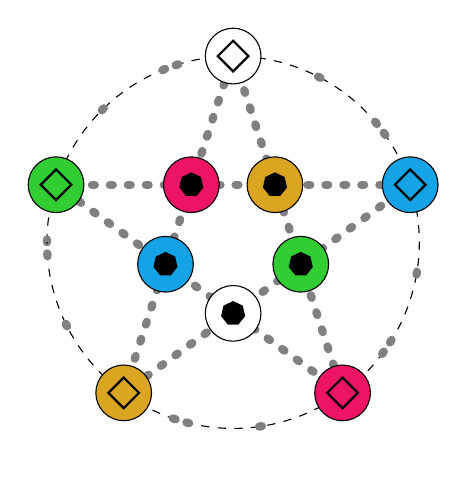
\begin{tikzpicture}[scale=0.65]

    \scriptsize
    \begin{scope}[xscale=-1]

    \boardy

    
    \node[statez, fill=white] (1t) at (1) {};  
     
    \node[stateb, fill=black] (1b) at (1a) {}; 
     
    \node[statez, fill=Cerulean] (2t) at (2){};   
     
    \node[stateb, fill=black] (2b) at (2a) {}; 
      
    \node[statez, fill=WildStrawberry] (3t) at (3) {};      
    
    \node[stateb, fill=black] (3a) at (3a) {}; 
    
    \node[statez, fill=Goldenrod] (4t) at (4) {};     
     
    \node[stateb, fill=black] (4a) at (4a) {}; 

    \node[statez, fill=LimeGreen] (5t) at (5) {};           
     
    \node[stateb, fill=black] (5b) at (5a) {};     
    
    \end{scope}
\end{tikzpicture}
   
    Put \textbf{black blocks on the crossings.}
    
    They are neutral.
    
    
\begin{tikzpicture}[scale=0.65]
        \node[stateb, fill=gray] (g1) at (-2,-6) {}; 
        \node[stateb, fill=gray] (g1) at (-1,-6) {}; 
        \node[stateb, fill=gray] (g1) at (0,-6) {}; 
        \node[stateb, fill=gray] (g1) at (1,-6) {}; 
        \node[stateb, fill=gray] (g1) at (2,-6) {}; 
            
\end{tikzpicture}

    Safe \textbf{grey blocks} for later.
  
\newpage
  
\skipper 

 

\begin{tikzpicture}[scale=0.65]
    \scriptsize
    \begin{scope}[xscale=-1]

    \boardy

    \draw[>=triangle 45, line width=1.5pt, ->] ({360/\n * (1-1)+95}:\radius)  arc ({360/\n * (1-1)+95}:{360/\n * (2-1)+80}:\radius) node[midway,left]{};
    
    \draw[>=triangle 45, line width=1.5pt, ->] ({360/\n * (1-1)+95}:\radius)  arc ({360/\n * (1-1)+95}:{360/\n * (-1)+100}:\radius) node[midway,left]{};
    

    
    
    
    \node[statez, fill=white] (1t) at (1) {};  
    
    \draw[>=triangle 45, line width=1.5pt, shorten >=1.5ex, ->] (1t) -- (4a);
    
    \draw[>=triangle 45, line width=1.5pt, shorten >=1.5ex, ->] (1t) -- (3a);    
   
    \end{scope}
\end{tikzpicture}
    
    You can move \textbf{in any direction,} on the ring and on the star.
    
 \skipper

    \centering
\begin{tikzpicture}[scale=0.65]
    \scriptsize
    \begin{scope}[xscale=-1]

    \boardy 
    
    \node[statez, fill=white] (1t) at (1) {};  
    
    \node[stateb, fill=black] (1z) at (1a) {}; 
     
    \node[statez, fill=Cerulean] (2t) at (2){};   
    
    \node[stateb, fill=black] (2z) at (2a) {}; 
      
    \node[statez, fill=WildStrawberry] (3t) at (3) {};  
    
    \node[stateb, fill=black] (3z) at (3a) {};     
    
    \node[statez, fill=Goldenrod] (4t) at (4) {};     
     
    \node[stateb, fill=black] (4z) at (4a) {}; 
       
    \node[statez, fill=LimeGreen] (5t) at (5) {};       
     
    \node[stateb, fill=black] (5z) at (5a) {};     
    
    \draw[>=triangle 45, line width=1.5pt, shorten >=1.5ex, ->] (1t) -- (4a);
    \end{scope}
    \end{tikzpicture}
    
    You can move \textbf{as far as you want.}
    
    But:\textbf{ you cannot jump!}
    

\newpage    
   
\skipper

\begin{tikzpicture}[scale=0.65]
    \scriptsize
    \begin{scope}[xscale=-1]

    \boardy
       
    \node[staten] (1t) at (1) {};      
     
    \node[stateb, fill=black] (1z) at (1a) {}; 
     
    \node[stateb, fill=black] (2z) at (2a) {};
    
    \node[stateb, fill=black] (3a) at (3a) {};     
     
    \node[statez, fill=white] (4z) at (4a) {}; 
        
    \node[stateb, fill=black] (5z) at (5a) {};     
    
    \node[stateb, fill=black] (2l) at ({360/\n * (2.5 - 1)+90}:\radius){};
    
    \draw[>=triangle 45, line width=1.5pt, ->] (1t) -- (4z) node[midway,right]{$hit$};
    
    \draw[dashed, >=triangle 45, line width=1.5pt, ->] (4z) -- (2l) node[midway,right]{$replace$};
    
    \end{scope}
\end{tikzpicture}
    
    You can \textbf{hit a black block.} 
    
    You then \textbf{replace} it on another empty space.
    
  
\skipper

\begin{tikzpicture}[scale=0.65]
    \scriptsize
    \begin{scope}[xscale=-1]

    \boardy

    \node[statez, fill=Cerulean] (1t) at (1) {};      
    
    \node[statez, fill=white] (2t) at (2){};       
    
    \draw[>=triangle 45, style=double, double distance=2pt, line width=0.5pt, <->] ({360/\n * (1-1)+95}:\radius)  arc ({360/\n * (1-1)+95}:{360/\n * (2-1)+85}:\radius) node[midway,right]{$swap$};
    
    \end{scope}
    \end{tikzpicture}
    
    You can \textbf{swap} two neighbouring pieces \\ (at least one of which must be yours). 
    
    Of course the way must be free!
    
    
\newpage    
\skipper
    
    
\begin{tikzpicture}[scale=0.65]
    \scriptsize
    \begin{scope}[xscale=-1]

    \boardy
    
    \node[staten] (1n) at (1) {};  
     
    \node[statez, fill=white] (1t) at (1a) {};     
    
    \node[stateb, fill=gray] (2l) at ({360/\n * (2.5 - 1)+90}:\radius){};
    \node[staten] (2q) at ({360/\n * (2.5 - 1)+90}:\radius+50){};
    
    \draw[dashed, >=triangle 45, line width=1.5pt, ->] (1n) -- (1t);
    
    \draw[>=triangle 45, line width=1.5pt, ->] (1t) -- (6,-1) node[left]{out};
    
    \draw[>=triangle 45, line width=1.5pt, <-] (2l) -- (2q) node[right] {in};
    
    \end{scope}
\end{tikzpicture}
    
    When you \textbf{reach a goal,} your piece moves \textbf{out. }
    
    (Three out wins!)
    
    For this you \textbf{place a grey block} anywhere.
    
    Grey blocks are \textbf{one-time blocks.}
    
    When you beat them, you remove them again.
    
  
\skipper


\begin{tikzpicture}[scale=0.65]
    \scriptsize
    \begin{scope}[xscale=-1]

    \boardy
    
    \node[staten] (1n) at (1) {};  
     
    \node[statez, fill=white] (1t) at (1a) {}; 
    
    \node[stateb, fill=black] (2t) at (2){};       
     
    \node[stateb, fill=black] (2z) at (2a) {}; 
      
    \node[stateb, fill=black] (3t) at (3) {};      
    
    \node[stateb, fill=black] (3z) at (3a) {};     
    
    \node[stateb, fill=black] (4z) at (4) {};     
       
    \node[stateb, fill=black] (5z) at (5) {};       
     
    \node[inner sep=0pt,outer sep=0,draw] (5n) at (5a) {}; 
    
    \draw[>=triangle 45, line width=1.5pt, -] (1n) -- (5n) node[midway,right]{};
    \draw[>=triangle 45, line width=1.5pt, ->] (5n) -- (1t) node[midway,left]{};
    
    \end{scope}
    \end{tikzpicture}
    
    \textbf{Turn} at free corners without stopping. 

    Ways can be long!
    
\newpage
    
\skipper
    
    \textbf{3:2}
    
\begin{tikzpicture}
    \node[alice, minimum size=1cm] at (-1,2) (alice) {};
    \node[statez, fill=white] at (1,2) {};
    \node[statez, fill=Cerulean] at (2,2) {};
    \node[statez, fill=WildStrawberry] at (3,2) {};
    \node at (5,2) {\textbf{3}} ;
    \node at (6,2) {\checkmark};

    \node[bob, minimum size=1cm] at (-1,0) (bob) {};
    \node[statezz, fill=WildStrawberry] at (1,0) {};
    \node[statezz, fill=LimeGreen] at (2,0) {};
    \node at (5,0) {\textbf{2}} ;
    \node at (6,0) {\textbf{-}} ;

\end{tikzpicture}
        
    The winner is who gets \textbf{three} pieces to their goals.


\skipper

    \raggedright
    
    \vspace{5ex}
    
    \textbf{Edge cases:}

    \begin{enumerate}
        \item When moving to a corner with multiple pieces, swap with one of them.
        \item When you get to set both a grey and a black block say `abracadabra'.
        \item You are not allowed to try the exact same move twice.        
  %      \item You cannot move out when it is not your turn.
        \item When one of your pieces was brought to its goal by someone else, then you must move that piece out when it is your turn and you set a grey block.\\ You do not gain an extra move.
        \item If you need more grey blocks than there are, re-position one.
    \end{enumerate}

\hrulefill


\vspace{5ex}

\begin{centering}
    This is the whole of the law.
\end{centering}

\vfill

\begin{framed}
\centering

\textbf{Warning: }This game is addictive.

If you experience anything unusual, please get in touch:

\href{mailto:jan@pentagame.org}{jan@pentagame.org}

\end{framed}
